\chapter[Processo de Integração]{\textbf{P}rocesso de \textbf{I}ntegração}
\addcontentsline{toc}{chapter}{Processo de Integração}

\textit{Neste capítulo são apresentados os procedimentos para a integração dos sistemas envolvidos, expondo o detalhes de implementação e configuração da solução proposta.}


\section{Definição da Solução}

Após o estudo aprofundado sobre o sistema GSAN e software Asterisk foram identificadas diversas formas de realizar a integração, entre os sistemas pelo fato da existência de várias protocolos possíveis de comunicação , no entanto a solução adotada será visando a reusabilidade, baixo custo de manutenção e o uso de tecnologias que já tenham uma maturidade no mercado. Foram escolhidos os protocolos SOAP e AGI para serem implementados por um \textit{Middleware}, este será responsável em assumir o papel de intermediário entre os sistemas GSAN e Asterisk. Com o intuito de facilitar o entendimento da comunicação entre os sistemas, a seguir será exposto o diagrama de implantação da solução (figura \ref{figura:diagramaImplantacao}) descrita acima, explanado os principais detalhes adotados nesta integração:


\begin{figure}[H]
	\centering
	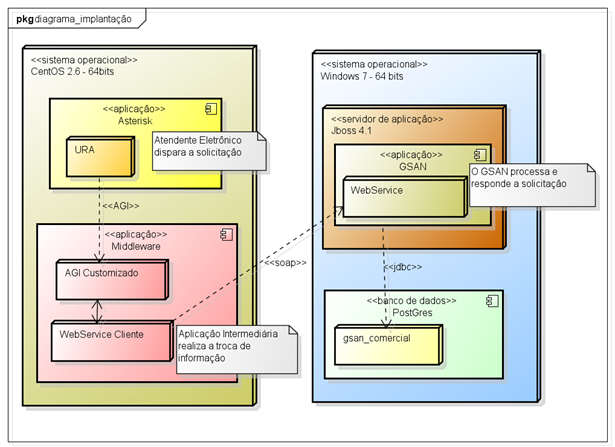
\includegraphics{figuras/diagrama_implantacao.png}
	\caption{Diagrama de implantação da solução}
	\label{figura:diagramaImplantacao}	
	Fonte – Autoria Própria
\end{figure}


Conforme ilustrado acima, o sistema GSAN irá prover uma interface de serviços na forma de WebServices utilizando o protocolo de comunicação SOAP (\textit{Simple Object Access Protocol}), tais serviços serão consumidos através do \textit{Middleware} intermediário denominado integrador que além de consumir os serviços do sistema GSAN, deverá também prover uma interface de serviços na forma utilizando o protocolo AGI, para então ser consumidos pelo Asterisk e responder a solicitação da Unidade de Resposta Audível.


\section{Tecnologias Utilizadas}
O processo de integração será composto por tecnologias com paradigmas diferenciados, no entanto para melhorar o entendimento dos detalhes de compatibilidades adotados segue abaixo a tabela \ref{tabela:tecnologiasUtilizadas}
	 das tecnologias utilizadas e versões correspondentes.


\begin{table}[H]
	\center
	\footnotesize
	\begin{tabular}{|p{4cm}|p{7cm}|p{2cm}|}
		\hline
		\textbf{Software} & \textbf{Finalidade} & \textbf{Versão} \\
		\hline
		Java Platform, \textit{Enterprise Edition} 5 (JEE) & Conjunto de Tecnologias e Serviços para implementar soluções da Plataforma Java com estabilidade, segurança e escalabilidade. & 5 \\
		\hline
		JBoss & Servidor de aplicação que implementa especificações JEE. & 4.0.1 sp1 \\
		\hline
		Hibernate & Framework utilizado para fazer o mapeamento objeto-relacional. É responsável pela camada de persistência. & 3.1 \\
		\hline
		PostgreSQL & Banco de dados relacional. & 9.3.4 \\
		\hline
		Apache Ant & Geração de \textit{Enterprise Application Resources} (EAR) deploy’s. & 1.6.2 \\
		\hline
		JasperReports & Tecnologia utilizada para criação de relatórios em PDF, HTML, XLS, CSV e XM.L & 1.2.2 \\
		\hline
		Struts & Framework para controle de navegação e validação Web. & 1.1	 \\
		\hline
		Disc-OS & Distribuição CentOS 2.6 que implementa interface web para a ferramenta Asterisk. & 2.0-1 \\
		\hline
		Asterisk & Software livre que permite a criação de PABX com diversos recursos. & 1.4 \\		
		\hline
		Asterisk-Java & Framework para comunicação com o Asterisk via protocolo AGI. & 1.0 \\	
		\hline			
	\end{tabular}
	\caption{Tecnologias utilizadas}
	\label{tabela:tecnologiasUtilizadas}
	Fonte – Autoria Própria
\end{table}



\section{Etapas da Integração}
O processo de integração entre os sistemas será composto por três etapas principais, das quais serão necessários para compor a solução escolhida, conforme definido abaixo e descrito nas sessões seguintes:

\begin{itemize}
	\item Implementar WebServices no Sistema GSAN 
	\item Desenvolver Middleware
	\item Customizar o Asterisk	
\end{itemize}
